\epi{I'm always delighted by the light touch and stillness of
early programming languages.  Not much text; a lot gets
done. Old programs read like quiet conversations
between a well-spoken research worker and a well-
studied mechanical colleague, not as a debate with a
compiler.  Who'd have guessed sophistication bought
such noise?}{\textsc{Dick Gabriel}}

\noindent{}Functions are the basic building blocks in Go programs; all interesting
stuff happens in them. A function is declared as follows:
\begin{lstlisting}[caption=A function declaration,label=src:function definition]
|\begin{tikzpicture}[overlay]
\ubrace{0.6,-1.5}{0.0,-1.5}{The keyword \key{func} is used to declare a function;}
%
\ubrace{2.2,-1.5}{0.8,-1.5}{A function can be defined to work on a specific type, a %
more common name for such a function is \index{method}{method}. This part is %
called a \first{\emph{receiver}}{receiver} and it is optional. See %
chapter \ref{chap:interfaces};}
%
\ubrace{3.4,-1.5}{2.4,-1.5}{\emph{funcname} is the name of your function;}
%
\ubrace{4.5,-1.5}{3.6,-1.5}{The variable \var{q} of type \type{int} is %
the input parameter. The parameters are passed %
\first{\emph{pass-by-value}}{pass-by-value} meaning they are copied. %
But be aware that reference types (slices, channels, maps and interfaces) are %
\first{\emph{pass-by-reference}}{pass-by-reference} even though you %
do not see the pointers directly in the code;}
%
\ubrace{6.0,-1.5}{4.9,-1.5}{%
The variables \var{r} and \var{s} are the %
\index{named return parameters}{named return parameters} for this function. %
Note that functions in Go can have multiple return values. See section %
"\titleref{sec:multiple return}" on page \pageref{sec:multiple return} %
for more information. If you want the return %
parameters not to be named you only give the types: %
\lstinline{(int,int)}. If you have only one value to return you may omit %
the parentheses. If your function is a subroutine and does not have %
anything to return you may omit this entirely;}
%
\ubrace{8.2,-1.5}{6.3,-1.5}{This is the function's body, note that %
\func{return} is a statement so the braces around the parameter(s) are %
optional.}
\end{tikzpicture}|
type mytype int	|\coderemark{New type, see chapter \ref{chap:beyond}}|

func (p mytype) funcname(q int) (r,s int) { return 0,0 }
||
\end{lstlisting}

\showremarks
Here are a two examples, the first is a function without a return value,
the second is a simple function that returns it's input.
\begin{lstlisting}
func subroutine(in int) {
    return
}
\end{lstlisting}
\begin{lstlisting}
func identity(in int) int {
    return in
}
\end{lstlisting}
One thing that is now allowed in Go is functions in functions. 
\begin{lstlisting}
func a() {
    println("Hello from a()")
    func b() {			    |\coderemark{Illegal nesting}|
	println("Hello from b()")    
    }
}
\end{lstlisting}
You can however
work around this by using anonymous functions (see section
"\titleref{sec:functions as values}" on page \pageref{sec:functions as values} 
in this chapter).

\section{Scope}
Variables declared outside any functions are global in Go, those
defined in functions are local to those functions. If names overlap --- a
local variable is declared with the same name as a global one --- the
local variable masks the global one when the current function is
executed.
\begin{minipage}{.5\textwidth}
\begin{lstlisting}[linewidth=.5\textwidth,caption=Local scope]
|\begin{tikzpicture}[overlay]
\draw [->,thick] (3.1,-5.00) arc (-60:90:2.00cm);
\draw [->,thick] (3.1,-7.00) arc (-60:90:0.20cm);
\end{tikzpicture}|
package main

var a = 6

func main() {
        p()
        q()
        p()
}

func p() {
        println(a)
}

func q() {
        a := 5
        println(a)
}
\end{lstlisting}

\hfill
\vfill
\end{minipage}
\begin{minipage}{.5\textwidth}
\begin{lstlisting}[caption=Global scope,label=src:scope2]
|\begin{tikzpicture}[overlay]
\draw [->,thick] (2.8,-5.00) arc (-60:90:2.00cm);
\draw [->,thick] (3.4,-7.00) arc (-60:90:3.15cm);
\end{tikzpicture}|
package main

var a = 6

func main() {
    p()
    q()
    p()
}

func p() {
    println(a)
}

func q() {
    a = 5|\coderemark{Assignment}|
    println(a)
}
\end{lstlisting}

\hfill
\vfill
\end{minipage}

In listing \ref{src:scope1} we introduce a local variable \var{a}
in the function \func{q()}
This local \var{a} is only visible in \func{q()}. That is
why the code will print: \texttt{656}.
In listing \ref{src:scope2} no new variables are introduced, there
is only a global \var{a}.
Assigning a new value to it is globally visible. This code will
print: \texttt{655}

In the following example we call \func{g()} from \func{f()}:
\lstinputlisting[caption=Scope when calling functions from functions]{src/scope3.go}
And this will print: \texttt{565}. So a \emph{local} variable is only
valid when we are executing the function in which it is defined. One
remaining case has not been dealt with and that is a "function
literal" in which you essentially define a function inside another
function. The following figure should clarify why it
prints:\texttt{565757}. \emph{Hint}: Just follow the arrows.

\begin{lstlisting}[caption=Scope and function literals,label=src:scope3,float]
|\begin{tikzpicture}[overlay]
\draw [->,thick] (2.8,-4.10) arc (-60:90:0.20cm);
\draw [->,thick] (2.8,-2.00) arc (-60:90:0.20cm);
\draw [->,thick] (2.4,-1.60) arc (-60:90:0.50cm);
%
\draw [->,thick] (4.4,-8.75) arc (-60:80:4.30cm);
% function f()
\draw [->,thick] (4.4,-5.85) arc (-60:90:0.30cm);
\draw [->,thick] (4.4,-5.25) arc (-60:90:0.90cm);
%
\draw [->,thick] (3.2,-7.45) arc (-60:65:2.00cm);
\end{tikzpicture}|
package main
var a int
func main() {
        a = 5
        println(a)
        f()
}
func f() {
        a := 6
        println(a)
        g()
        x := func() {
                a = 7
                println(a)
        }
        x()
        g()
        println(a)
}
func g() {
        println(a)
}
\end{lstlisting}


\section{Multiple return values}
\label{sec:multiple return}
One of Go's unusual features is that functions and methods can return multiple
values. This can be used to improve on a couple of clumsy idioms in C programs:
in-band error returns (such as -1 for \texttt{EOF}) and modifying an argument.

In C, a write error is signaled by a negative count with the error code
secreted away in a volatile location. In Go, \lstinline{Write} can return a count and an
error: "Yes, you wrote some bytes but not all of them because you filled the
device". The signature of \lstinline{*File.Write} in package
\package{os} is:
\begin{lstlisting}
func (file *File) Write(b []byte) (n int, err Error)
\end{lstlisting}
and as the documentation says, it returns the number of bytes written and a
non-\lstinline{nil} Error when \lstinline{n != len(b)}. This is a common
style in Go.

A similar approach obviates the need to pass a pointer to a return value to
simulate a reference parameter. Here's a simple-minded function to grab a
number from a position in a byte array, returning the number and the next
position.
\begin{lstlisting}
func nextInt(b []byte, i int) (int, int) {
    for ; i < len(b) && !isDigit(b[i]); i++ {
    }
    x := 0
    for ; i < len(b) && isDigit(b[i]); i++ {
        x = x*10 + int(b[i])-'0'
    }
    return x, i
}
\end{lstlisting}
You could use it to scan the numbers in an input array a like this:
\begin{lstlisting}
    for i := 0; i < len(a); {
        x, i = nextInt(a, i)
        fmt.Printf("%d", x)
    }
\end{lstlisting}
With having tuples as a native type, multiple return values is the next
best thing to have. You can return precisely what you want without
overloading the domain space with special values to signal errors.

\section{Named result parameters}
\label{sec:named result parameters}
The return or result "parameters" of a Go function can be given names and used
as regular variables, just like the incoming parameters. When named, they are
initialized to the zero values for their types when the function begins; if the
function executes a \key{return} statement with no arguments, the current values of
the result parameters are used as the returned values. Using this
features enables you (again) to do more with less code\footnote{This is
sort of a motto of Go; "Do more, with less code".}.

The names are not mandatory but they can make code shorter and clearer:
\emph{they are documentation}. 
If we name the results of \lstinline{nextInt} it becomes obvious which
returned \type{int} is which.

\begin{lstlisting}
func nextInt(b []byte, pos int) (value, nextPos int) {
\end{lstlisting}
Because named results are initialized and tied to an unadorned
\key{return},
they can simplify as well as clarify. Here's a version of
\lstinline{io.ReadFull} that uses them well:

\begin{lstlisting}
func ReadFull(r Reader, buf []byte) (n int, err os.Error) {
    for len(buf) > 0 && err == nil {
        var nr int
        nr, err = r.Read(buf)
        n += nr
        buf = buf[nr:len(buf)]
    }
    return
}
\end{lstlisting}

In the following example we declare a simple function which calculates
\gomarginpar{Some text in this chapter comes from \cite{go_intro}.}  % layout
the factorial value of a value \var{x}.

\begin{lstlisting}
func Factorial(x int) int { |\coderemark{\texttt{func Factorial(x int) (int)} is also OK}|
   if x == 0 {
      return 1;	
   } else {
      return x * Factorial(x - 1);
   }
}
\end{lstlisting}

When we use named result values, the code become indeed shorter and
more easy to understand.
So you could also write factorial as:
\begin{lstlisting}
func Factorial(x int) (result int) {
  if x == 0 {
    result = 1;	
  } else {
    result = x * Factorial(x - 1);
  }
  return;
}
\end{lstlisting}
You can also write the function with multiple return values:

\begin{lstlisting}
func fib(n) (val int, pos int) {
   if n == 0 {
      val = 1;
      pos = 0;
   } else if n == 1 {
      val = 1;
      pos = 1;
   } else {
      v1, _ := fib(n-1);
      v2,_ := fib(n-2);
      val = v1 + v2;
      pos = n;
   }
   return;
}
\end{lstlisting}

\section{Deferred code}
Suppose you have a function in which you open a file and perform various
writes and reads on it. In such a function there are often spots where
you want to return early. If you do that, you will need to close the file
descriptor you are working on. This often leads to the following code:
\begin{lstlisting}[caption=Without \func{defer}]
function ReadWrite() bool {
    file.Open("file")
    // Do you thing
    if failureX {
	file.Close("file")
	return false
    }

    if failureY {
	file.Close("file")
	return false
    }
    file.Close("file")
    return true
}
\end{lstlisting}
Where a lot of code is repeated, but with a good reason. To overcome this ---
and do more in less code --- Go has the \func{defer} statement. After
\func{defer} you specify a function which is called just \emph{before} a
return from the function is executed.

The above code could be rewritten with it as follows, making the whole
function more readable, shorter and puts the \func{Close} right next 
to the \func{Open}.
\begin{lstlisting}[caption=With \func{defer}]
function ReadWrite() bool {
    file.Open("file")
    defer file.Close("file") |\coderemark{\func{file.Close} \emph{is} the function}|
    // Do you thing
    if failureX {
	return false	     |\coderemark{\func{Close} is now done automatically}|
    }
    if failureY {
	return false	     |\coderemark{And here too}|
    }
    return true
}
\end{lstlisting}
You can put multiple functions on the "deferred list", like this
example from \cite{effective_go}:
\begin{lstlisting}
for i := 0; i < 5; i++ { 
    defer fmt.Printf("%d ", i) 
} 
\end{lstlisting}
Deferred functions are executed in LIFO order, so the above code
prints: \lstinline{4 3 2 1 0}. 

With \func{defer} you can even change return values, provided that
you are using named result parameters and a function literal, i.e:
\begin{lstlisting}[caption=Function literal]
defer func() {
	...
}()		 |\coderemark{() is needed here}|
\end{lstlisting}
In that (unnamed) function you can access any named return
parameter like so:
\begin{lstlisting}[caption=Access return values within \func{defer}]
func f() (ret int){     |\coderemark{\var{ret} is initialized with %
zero}|
	defer func() {
		ret++	|\coderemark{Increment \var{ret} with $1$}|
	}()
	return 0	|\coderemark{$1$ \emph{not} $0$ will be returned}|
}
\end{lstlisting}


\section{Variadic parameters}
Functions that take variadic parameters are functions that have a
variable number of parameters. In Go this is done as follows.
Firstly you need to declare your function to take variadic arguments:
\begin{lstlisting}[caption=Variadac parameters]
func myfunc(arg ... int) {}
\end{lstlisting}
The \lstinline{arg ... int} instructs Go to see this as a function that
takes a variable number of arguments. Note that all these arguments
have the type \type{int}. Inside your function's body the variable
\var{arg} is a slice of \type{int}s:
\begin{lstlisting}
for _, n := range arg {
    fmt.Printf("And the number is: %d\n", n)
}
\end{lstlisting}

If you don't specify the type of the variadac argument it defaults to the
empty interface \var{interface\{\}}.

\section{Functions as values}
\label{sec:functions as values}
As with almost everything in Go, functions are also \emph{just} values,
so they can be assigned to variables. Like so:
\lstinputlisting[label=src:anonfunc,caption=Anonymous function]{src/anon-func.go}
If we use \lstinline{fmt.Printf("%T\n", a)} to print the type of \var{a} it prints
\func{func()}.

Functions--as--values may also be used in other places, like in maps.
This code is from the package \package{net} (in the file
\package{net/dnsmsg.go}), where a map is used to convert
from integers to functions.
\begin{lstlisting}[caption=Function as values in maps]
var rr_mk = map[int]func() dnsRR{
    dnsTypeCNAME: func() dnsRR { return new(dnsRR_CNAME) },
    dnsTypeHINFO: func() dnsRR { return new(dnsRR_HINFO) },
    dnsTypeMB:    func() dnsRR { return new(dnsRR_MB) },
    ...
\end{lstlisting}


\section{Exercises}
\begin{Exercise}[title={Stack},difficulty=5]
\label{ex:stack}
\Question \label{ex:stack q1} Create a simple stack which can hold a
fixed amount of \key{int}s. Is does not have to grow beyond this limit.
Define both a \func{push} and \func{pop} function.

\begin{wrapfigure}{l}{30mm}
\begin{center}
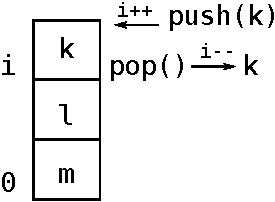
\includegraphics[scale=0.50]{fig/stack.pdf}
\end{center}
\end{wrapfigure}

\Question \label{ex:stack q2} Bonus. Write a \func{String} method which 
converts the stack to a string. This way you can print the stack using:
\lstinline{fmt.Printf("My stack %v\n", stack)}. This may aid in
debugging.
\end{Exercise}

\begin{Answer}

\Question 

\Question 

\end{Answer}


\begin{Exercise}[title={Stack as package},difficulty=2]
\label{ex:stack-package}
\Question\label{ex:stack-package q1} Create a proper package for your
stack implementation, \func{push}, \func{pop} and the \type{stack} type need to be
exported.

\Question\label{ex:stack-package q2} Which official Go package could
also be used for a (FIFO) stack?

\end{Exercise}

\begin{Answer}
\Question There are a few details that should be changed to make a proper package
for our stack. First, the exported function should begin with a capital 
letter and so should \type{Stack}. So the full package (including the
\func{String()} function becomes
\lstinputlisting[caption=Stack in a
package]{ex-functions/src/stack-as-package.go}

\Question The \package{container/vector} package would be a could candidate. It
even comes with \func{push} and \func{pop} functions \emph{predefined}.
\end{Answer}


\begin{Exercise}[title={Calculator},difficulty=7]
\label{ex:cacl}
\Question\label{ex:calc q1} Create a reverse polish calculator, use your
stack package.

\end{Exercise}

\begin{Answer}
\end{Answer}


\begin{Exercise}[title={Var args},difficulty=5]
\label{ex:varargs}
\Question\label{ex:varargs q1}
Write a function that takes a variable numbers of \type{int}s and prints
each integer on a seperate line
\end{Exercise}

\draft{BETER}
\begin{Answer}
\Question
For this we need the \lstinline{...}-syntax so signal we have a
function that takes an arbitrary number of arguments.

\lstinputlisting[label=src:varargs,caption=A function with variable number of arguments]{ex-functions/src/var-arg.go}

\end{Answer}


\begin{Exercise}[title={斐波那契},difficulty=5]
\label{ex:fibonaci}
\Question\label{ex:fibonaci q1}
斐波那契数列以:$1, 1, 2, 3, 5, 8, 13, \ldots$ 开始。
或者用数学形式表达:$ x_1 = 1; x_2 = 1; x_n = x_{n-1} +
x_{n-2}\quad\forall n > 2 $。

编写一个函数,接受 \type{int} 值,并给出这个值得到的斐波那契数列。

\end{Exercise}

\begin{Answer}
\Question
下面的程序会计算出斐波那契数列。
\lstinputlisting[label=src:fib,caption=Fibonacci function in Go]{ex-functions/src/fib.go}

\showremarks
\end{Answer}


\cleardoublepage
\section{Answers}
\shipoutAnswer
